\section{W8: Configuration Management}

\textbf{The role of configuration management.}

    \textbf{Establishing processes.}

    \textbf{Setting up repositories.}

    \textbf{Using other appropriate tools and techniques.}

\textbf{The configuration management process.}

    \textbf{To identify all items that collectively will make up the configuration.}

    \textbf{To manage changes to one or more of these items so that the collection remains consistent.}

    \textbf{To manage different versions of the product.}

    \textbf{To assure software quality as the configuration evolves over time.}

\textbf{The tasks associated with configuration management.}

    \textbf{Identification}: the configuration items necessary for the project are identified.

    \textbf{Version control}: processes and tools are chosen to manage the different versions of configuration items as they are developed.

    \textbf{Change control}: changes that affect more than just one configuration item are managed.

    \textbf{Configuration auditing}: the consistency of the configuration is checked.

    \textbf{Configuration/status reporting}: the status of the configuration items is reported.

    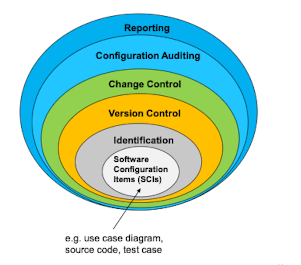
\includegraphics[width=\linewidth]{figs/SCR-20240606-pkfg.png}
